\section{Testphase}
	
	Ziel:		
	\begin{itemize}
		\item Softwarefehler möglichst \textbf{früh finden}
		\begin{itemize}
			\item \textbf{Zeit ist Geld!}
		\end{itemize}
	\end{itemize}
		
	\subsection{Fehlerarten}
		
		\begin{itemize}
			\item \textbf{Irrtum/Herstellungsfehler:} Menschliche Aktion, die zum Defekt führt
			\item \textbf{Defekt:} Mangel an Softwareprodukt
			\item \textbf{Versagen/Ausfall:} Abweichung des Softwareverhaltens
		\end{itemize}
			
	\subsection{Fehlerklassen}
	
		\begin{itemize}
			\item \textbf{Anforderungsfehler} (Defekt im Pflichtenheft)
			\begin{itemize}
				\item Inkorrekte Benutzerwünsche,..
			\end{itemize}
			\item \textbf{Entwurfsfehler} (Defekt in der Spezifikation)
			\begin{itemize}
				\item Unvollständige/fehlerhafte Umsetzung der Anforderung,..
			\end{itemize}
			\item \textbf{Implementierungsfehler} (Defekt im Programm)
			\begin{itemize}
				\item Fehlerhafte Umsetzung der Spezifikation im Programm,..
			\end{itemize}
		\end{itemize}
		
	\subsection{Arten von Testhelfern}
			
		\begin{itemize}
			\item \textbf{Stummel}: Rudimentär implementierter Softwareteil
			\item \textbf{Attrappe}: Simuliert die Implementierung zu Testzwecken
			\item \textbf{Nachahmung}: Attrappe mit zusätzlicher Funktion
		\end{itemize}
	
	\subsection{Testphasen}
			
		\begin{center}
			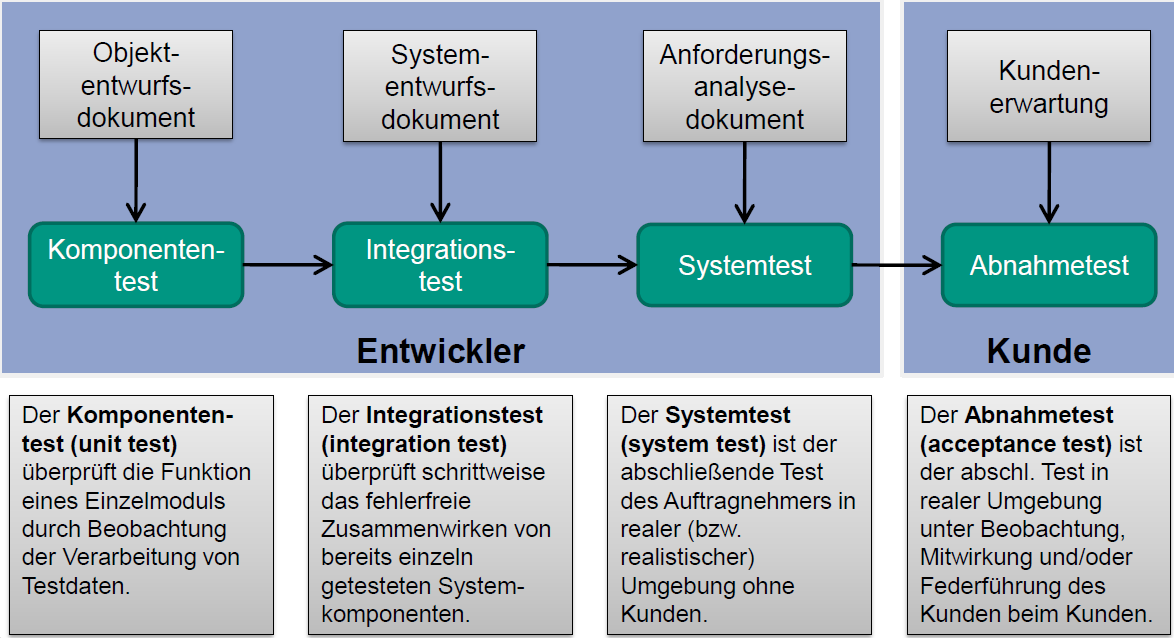
\includegraphics[width=0.8\textwidth]{../images/testphasen.png}
		\end{center}
		
	\subsection{Klassifikation testender Verfahren}
			
		\begin{itemize}
			\item \textbf{Dynamische Verfahren}
			\begin{itemize}
				\item Strukturtests
				\begin{itemize}
					\item Kontroll- und datenflussorientierte Tests
				\end{itemize}
				\item Funktionale Tests
				\item Leistungstests
			\end{itemize}
			\item \textbf{Statische Verfahren}
			\begin{itemize}
				\item Manuelle Prüfmethoden
				\item Prüfprogramme
			\end{itemize}
		\end{itemize}
			
		\newpage
		\subsubsection{Kontrollflussorientierte Testverfahren}
					
			\begin{itemize}
				\item \textbf{Anweisungsüberdeckung}
				\begin{itemize}
					\item Ausführung aller \textbf{Grundblöcke}
				\end{itemize}
				\item \textbf{Zweigüberdeckung}
				\begin{itemize}
					\item \textbf{Traversierung} aller Zweige
				\end{itemize}
				\item \textbf{Pfadüberdeckung}
				\begin{itemize}
					\item Ausführung aller \textbf{unterschiedlichen, vollständigen Pfade} im Programm
					\begin{itemize}
						\item Pfadanzahl \textbf{wächst bei Schleifen} enorm!
												
						$\Rightarrow$ \textbf{Nicht praktikabel!}
					\end{itemize}
				\end{itemize}
				\item Beispiel:
				\begin{center}
					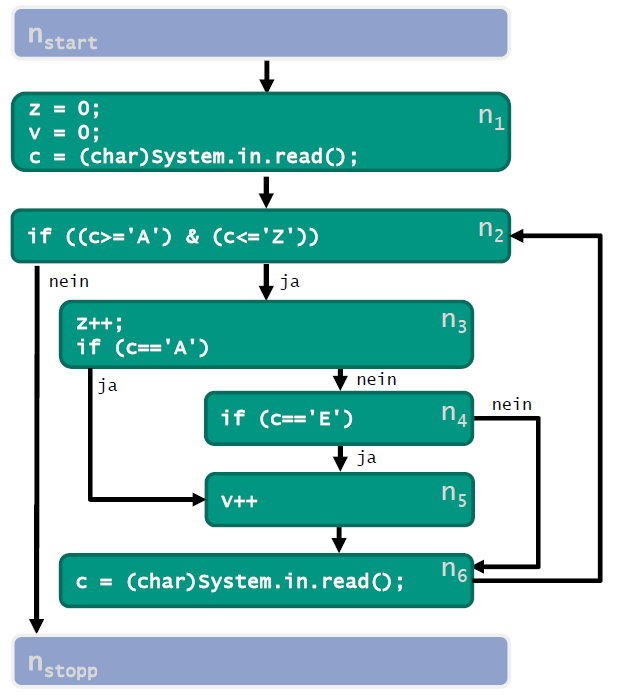
\includegraphics[width=0.6\textwidth]{../images/kfg.png}
				\end{center}
			\end{itemize}
	
		\subsubsection{Funktionale Tests}
			
			\begin{itemize}
				\item \textbf{Funktionale Äquivalenzklassenbildung}
				\begin{itemize}
					\item \textbf{Zerlege Wertebereich} der Eingabeparameter und \textbf{Definitionsbereich} der Ausgabeparameter in Äquivalenzklassen
				\end{itemize}
				\item \textbf{Grenzwertanalyse}
				\begin{itemize}
					\item Erweiterung von Äquivalenzklassenbildung mit \textbf{Grenzwerten}
				\end{itemize}
				\item \textbf{Zufallstest}
				\begin{itemize}
					\item \textbf{Zufällige Testfälle} (mit Testhelfern)
				\end{itemize}
				\item \textbf{Test von Zustandsautomaten}
				\begin{itemize}
					\item Testfälle aus \textbf{Zustandsübergängen}
				\end{itemize}
			\end{itemize}
		
		\subsubsection{Leistungstests}
				
			\begin{itemize}
				\item \textbf{Lasttests}
				\begin{itemize}
					\item Zuverlässigkeit und Einhalten der Spezifikation \textbf{im erlaubten Grenzbereich}
				\end{itemize}
				\item \textbf{Stresstests}
				\begin{itemize}
					\item Verhalten des System \textbf{beim Überschreiten} der definierten Grenzen
				\end{itemize}
			\end{itemize}
		
		\subsubsection{Manuelle Prüfung}
			
			\begin{itemize}
				\item \textbf{Semantik} wird geprüft
				\item \textbf{Aufwendig} (20\% der Erstellungskosten)
			\end{itemize}
	
		\subsubsection{Prüfprogramme}
				
			\begin{itemize}
				\item Warnungen, Fehler, Programmierstil, etc.
			\end{itemize}
	
		\subsubsection{Integrationstests}
			
			\begin{center}
				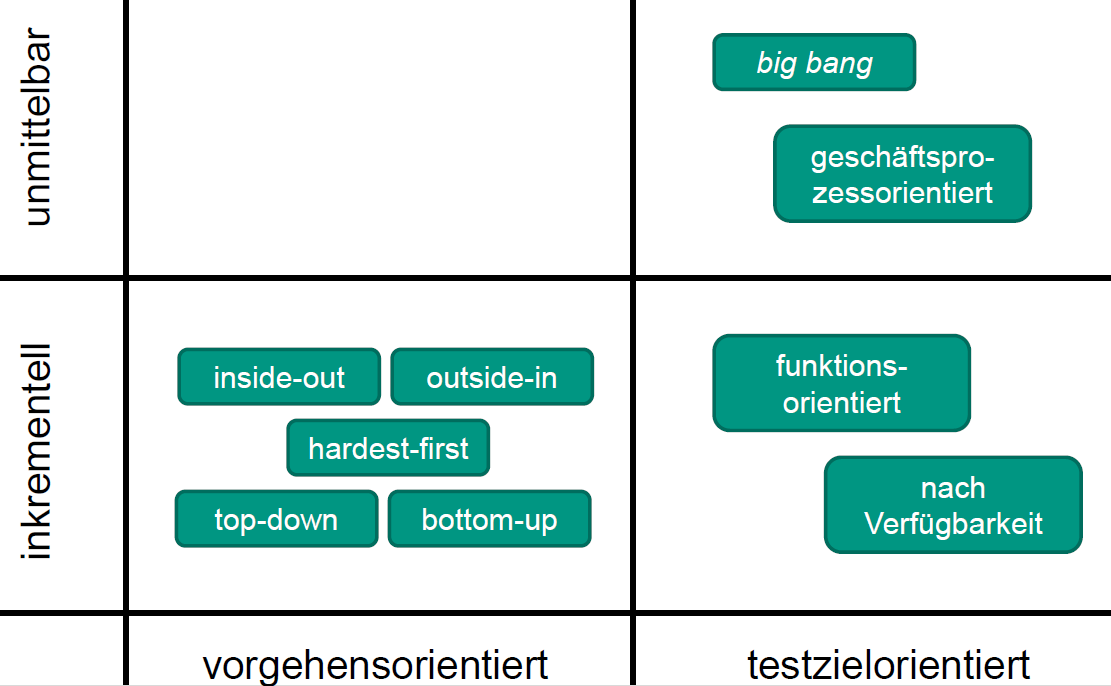
\includegraphics[width=0.6\textwidth]{../images/integrationstests.png}
			\end{center}
		
		\subsubsection{Systemtests}
				
			\begin{itemize}
				\item \textbf{Funktionaler Systemtest}
				\begin{itemize}
					\item Überprüfung funktionaler Qualitätsmerkmale, Korrektheit und Vollständigkeit
				\end{itemize}
				\item \textbf{Nichtfunktionaler Systemtest}
				\begin{itemize}
					\item Überprüfung nichtfunktionaler Qualitätsmerkmale wie: Sicherheit, Benutzbarkeit,..
				\end{itemize}
			\end{itemize}
		
		\subsubsection{Abnahmetests}
					
			\begin{itemize}
				\item Spezieller Systemtest: \textbf{Kunde beobachtet} oder \textbf{wirkt mit!}
				\item Formale Abnahme ist \textbf{bindende Erklärung der Annahme} durch den Auftraggeber
			\end{itemize}
		
	\subsection{Inspektion}
			
		\begin{itemize}
			\item \textbf{Phasen:}
			\begin{itemize}
				\item \textbf{Vorbereitung}
				\begin{itemize}
					\item \textbf{Teilnehmer/Rollen} festlegen
					\item \textbf{Dokumente/Formulare} vorbereiten
					\item \textbf{Zeitlichen Ablauf} planen
				\end{itemize}
				\item \textbf{Individuelle Fehlersuche}
				\begin{itemize}
					\item \textbf{Inspektoren prüfen} Dokumente für sich
					\item \textbf{Notieren der Problempunkte} und genaue Stelle im Dokument
					\item Problempunkte: Mögliche Defekte, Verbesserungsvorschläge, Fragen
				\end{itemize}
				\item \textbf{Gruppensitzung}
				\begin{itemize}
					\item \textbf{Problempunkte sammeln} und besprechen
					\item \textbf{Verbesserungsvorschläge sammeln}
				\end{itemize}
				\item \textbf{Nachbereitung}
				\begin{itemize}
					\item Liste der Problempunkte an \textbf{Editor}
					\item Editor identifiziert \textbf{tatsächliche Defekte} und \textbf{klassifiziert} sie
					\item \textbf{Alle Problempunkte} werden bearbeitet
				\end{itemize}
				\item \textbf{Prozessverarbeitung}
				\begin{itemize}
					\item \textbf{Standards für Dokumente} erarbeiten
					\item Defektklassifikationsschema, Planung und Durchführung verbessern
				\end{itemize}
			\end{itemize}
			\newpage
			\item \textbf{Rollen:}
			\begin{itemize}
				\item \textbf{Inspektionsleiter} (leitet alle Phasen)
				\item \textbf{Moderator} (leitet Gruppenphase)
				\item \textbf{Inspektor} (prüft Dokument)
				\item \textbf{Schriftführer} (protokolliert Defekte in Gruppensitzung)
				\item \textbf{Editor} (klassifiziert/behebt Defekte)
				\item \textbf{Autor} (verfasst Dokument)
			\end{itemize}
		\end{itemize}	
		\begin{center}
			\begin{tabular}{c|c}
				\color{green}{\textbf{+}}              & \color{red}{\textbf{-}} \\
				\hline
				- Anwendbar auf alle Softwaredokumente & - Aufwendig \\
				- Effektiv in industrieller Praxis     & - Teuer, da Zeitaufwand hoch \\
			\end{tabular}
		\end{center}